% !TeX root =Bachelorarbeit-Ziegenhagen.tex
\chapter{Einleitung}

\section{fsdfsdfs}

\blindtext[10]

\begin{figure}
\begin{center}
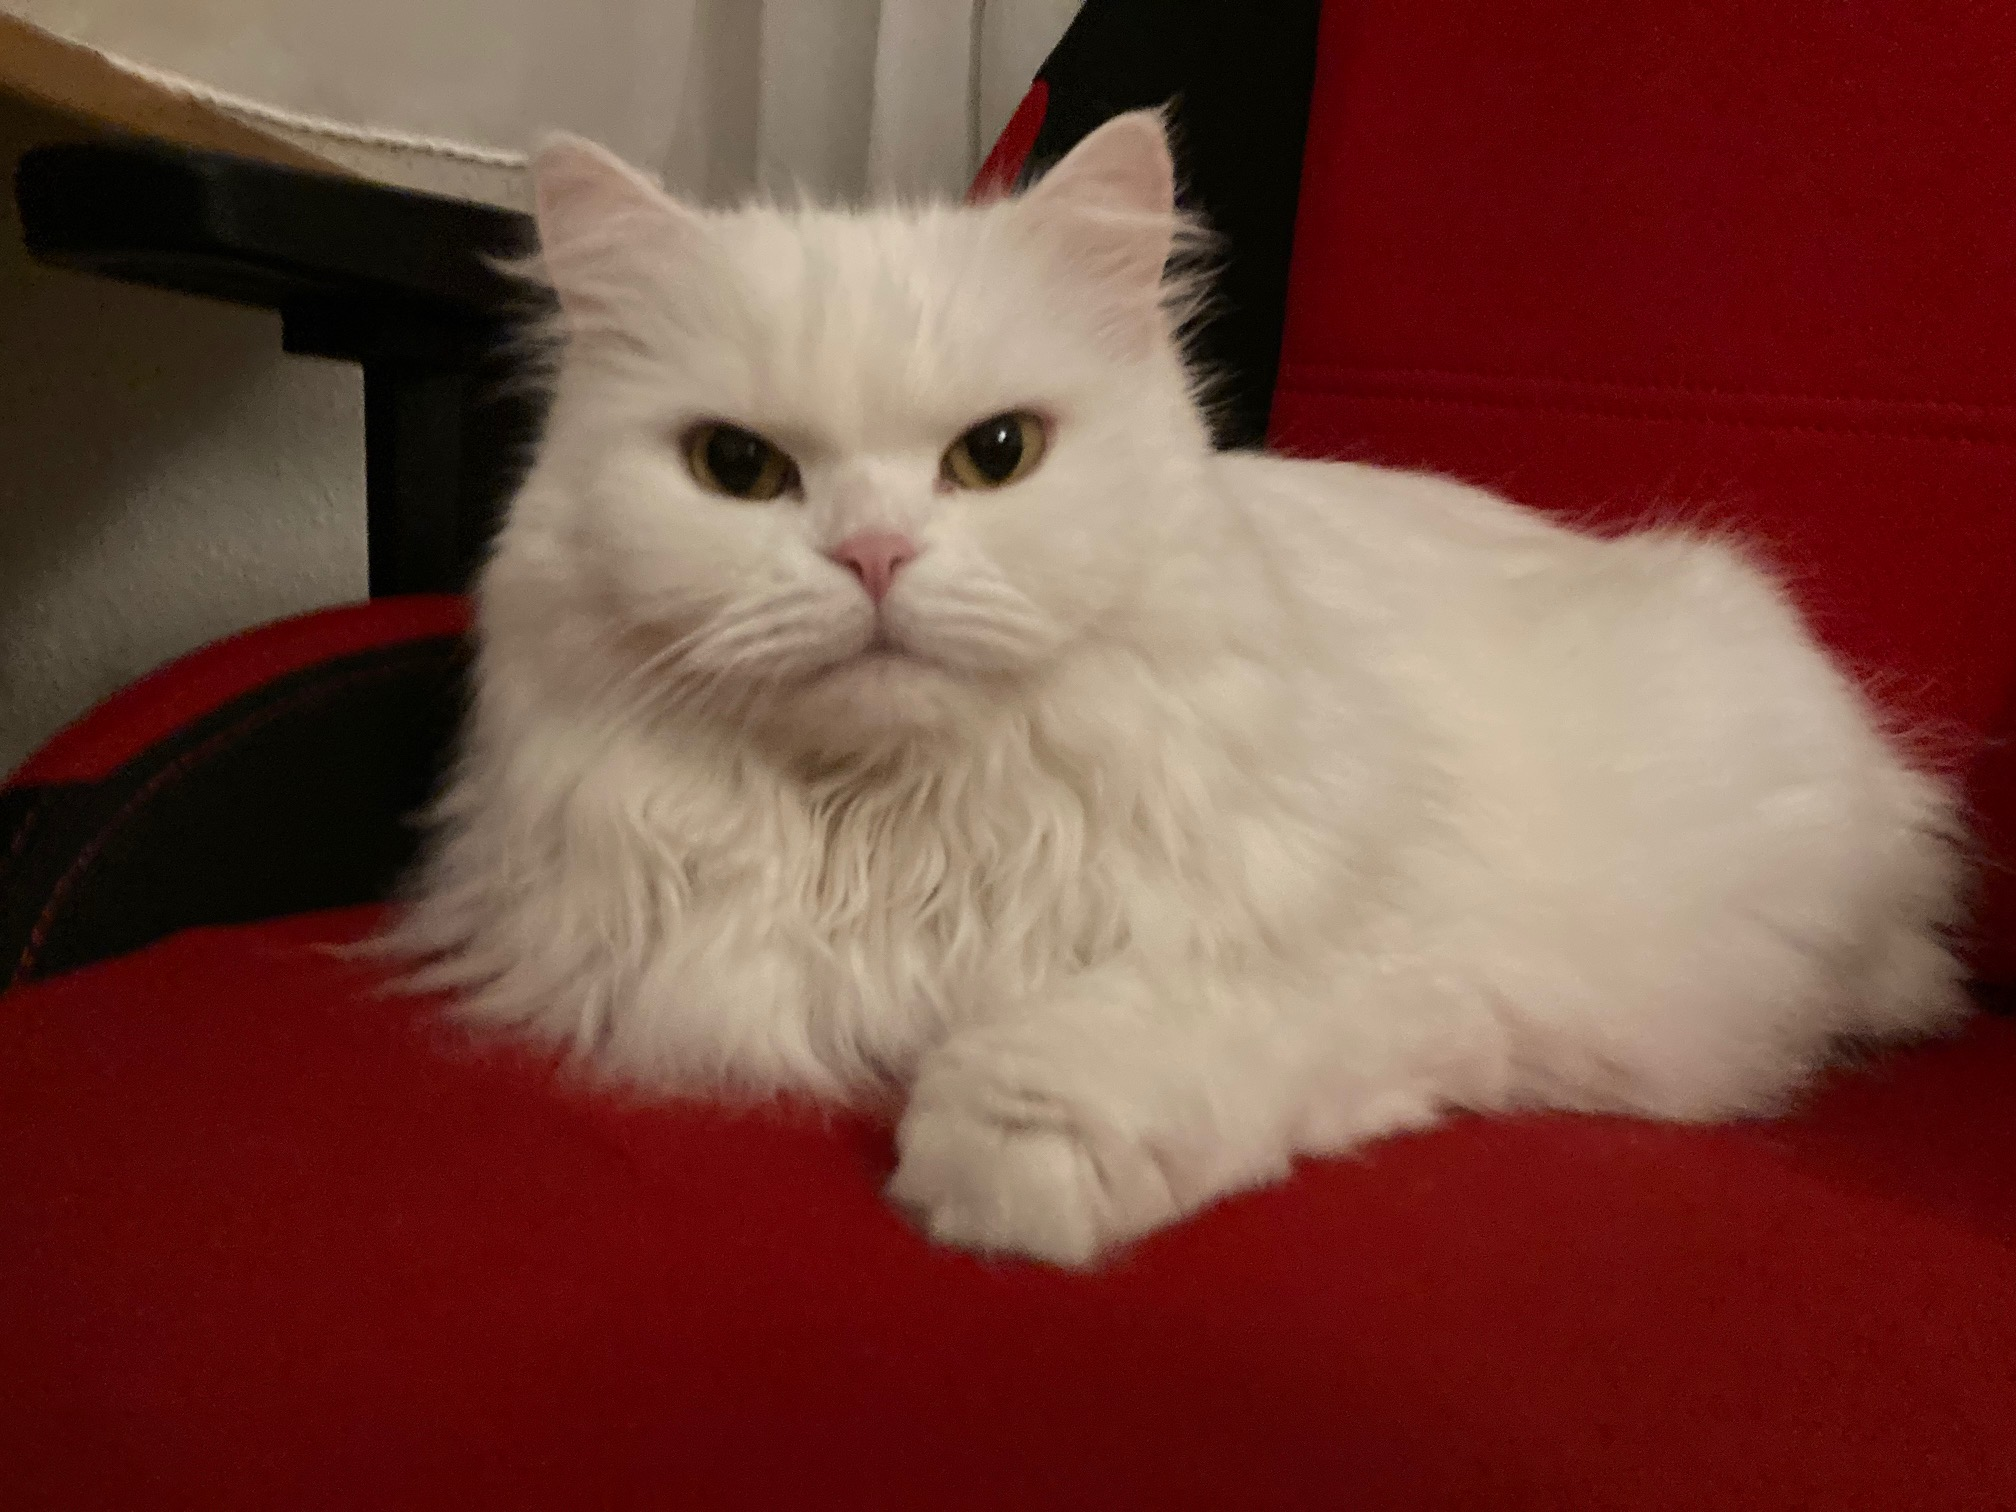
\includegraphics[width=0.8\textwidth]{Bilder/Katze.jpg}
\end{center}
\caption{Miezekatze}\label{fig:mieze}
\end{figure}


\blindtext[10]

\begin{itemize}
	\item wq
	\item eqwe
	\item qwe
	\item qwe
	\item qweqwe
	\item qwewe
\end{itemize}

\begin{compactitem}
	\item wq
	\item eqwe
	\item qwe
	\item qwe
	\item qweqwe
	\item qwewe
\end{compactitem}


\begin{enumerate}
	\item wq
	\item eqwe
	\item qwe
	\item qwe
	\item qweqwe
	\item qwewe
\end{enumerate}

\begin{compactenum}
	\item wq
	\item eqwe
	\item qwe
	\item qwe
	\item qweqwe
	\item qwewe
\end{compactenum}